\documentclass[12pt, twoside]{article}
\input{../preamble}

\fancyhead[LO]{La Scuola d'Italia / Dr.\ Huson / IB Math: Quiz \\* 13 March 2026}
\fancyhead[RO]{Markscheme}
\fancyfoot[C]{\thepage}

\begin{document}
\subsubsection*{4.19 Quiz: Probability (Algebra) --- Markscheme}

\begin{enumerate}[itemsep=0.15cm]

%--- Problem 1: Independence with algebra [6 marks] ---
\item Events $A$ and $B$ are independent. It is given that
      $\mathrm{P}(A) = 2\,\mathrm{P}(B)$ and $\mathrm{P}(A \cup B) = 0.72$.

      Let $x = \mathrm{P}(B)$.

\begin{enumerate}[itemsep=0.3cm]
  \item Show that $2x^{2} - 3x + 0.72 = 0$. \hfill [3]

  $\mathrm{P}(A \cup B) = \mathrm{P}(A) + \mathrm{P}(B) - \mathrm{P}(A \cap B)$ \hfill \textbf{(M1)}

  Since independent: $\mathrm{P}(A \cap B) = \mathrm{P}(A) \cdot \mathrm{P}(B) = 2x \cdot x = 2x^{2}$ \hfill \textbf{(M1)}

  $2x + x - 2x^{2} = 0.72$

  $2x^{2} - 3x + 0.72 = 0$ \hfill \textbf{(AG)}

  \emph{Note: final line must be shown with algebraic working, not just stated.} \hfill \textbf{(A1)}

  \item Hence find $\mathrm{P}(B)$. \hfill [2]

  $x = \dfrac{3 \pm \sqrt{9 - 4(2)(0.72)}}{2(2)}
     = \dfrac{3 \pm \sqrt{3.24}}{4}
     = \dfrac{3 \pm 1.8}{4}$ \hfill \textbf{(M1)}

  $x = 1.2$ (reject, $> 1$) or $x = 0.3$

  $\mathrm{P}(B) = 0.3$ \hfill \textbf{(A1)}

  \item Find $\mathrm{P}(A \cap B)$. \hfill [1]

  $\mathrm{P}(A \cap B) = \mathrm{P}(A) \cdot \mathrm{P}(B) = 0.6 \times 0.3 = 0.18$ \hfill \textbf{(A1)}
\end{enumerate}

\newpage

%--- Problem 2: Conditional probability + Venn [8 marks] ---
\item In a school, 80 students were surveyed about activities $A$ and $B$.

\begin{itemize}[itemsep=0.1cm]
  \item $\mathrm{P}(A) = 0.5$
  \item $\mathrm{P}(B \mid A) = 0.3$
  \item $\mathrm{P}(A' \cap B') = 0.2$
\end{itemize}

\begin{enumerate}[itemsep=0.3cm]
  \item Find $\mathrm{P}(A \cap B)$. \hfill [2]

  $\mathrm{P}(A \cap B) = \mathrm{P}(B \mid A) \times \mathrm{P}(A)$ \hfill \textbf{(M1)}

  $= 0.3 \times 0.5 = 0.15$ \hfill \textbf{(A1)}

  \item Find $\mathrm{P}(B)$. \hfill [2]

  $\mathrm{P}(A \cup B) = 1 - \mathrm{P}(A' \cap B') = 1 - 0.2 = 0.8$ \hfill \textbf{(M1)}

  $\mathrm{P}(B) = \mathrm{P}(A \cup B) - \mathrm{P}(A) + \mathrm{P}(A \cap B)
    = 0.8 - 0.5 + 0.15 = 0.45$ \hfill \textbf{(A1)}

  \item Complete the Venn diagram below, showing the number
        of students in each region. \hfill [2]

  $n(A \text{ only}) = 80 \times (0.5 - 0.15) = 80 \times 0.35 = 28$ \hfill \textbf{(A1)}

  $n(A \cap B) = 80 \times 0.15 = 12$

  $n(B \text{ only}) = 80 \times (0.45 - 0.15) = 80 \times 0.30 = 24$

  $n(\text{neither}) = 80 \times 0.2 = 16$ \hfill \textbf{(A1)}

\begin{center}
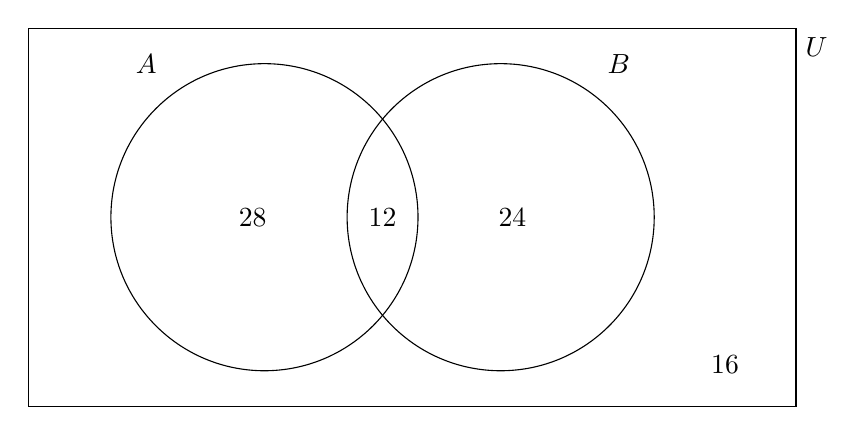
\begin{tikzpicture}[scale=1.5]
  \draw (0,0) rectangle (6.5,3.2);
  \draw (2.0,1.6) circle (1.3);
  \draw (4.0,1.6) circle (1.3);
  \node at (1.0,2.9) {$A$};
  \node at (5.0,2.9) {$B$};
  \node[anchor=north west] at (6.5,3.2) {$U$};
  \node at (1.9,1.6) {$28$};
  \node at (3.0,1.6) {$12$};
  \node at (4.1,1.6) {$24$};
  \node at (5.9,0.35) {$16$};
\end{tikzpicture}
\end{center}

  \item Determine whether events $A$ and $B$ are independent.
        Justify your answer. \hfill [2]

  $\mathrm{P}(A) \times \mathrm{P}(B) = 0.5 \times 0.45 = 0.225$ \hfill \textbf{(M1)}

  $\mathrm{P}(A \cap B) = 0.15$

  $0.225 \neq 0.15$, so the events are \textbf{not independent}. \hfill \textbf{(R1)}
\end{enumerate}

\bigskip
\noindent\textbf{Total: 14 marks}

\end{enumerate}
\end{document}
